\documentclass[aspectratio=169]{beamer}
\setbeamertemplate{navigation symbols}{}
\usepackage{color,amsmath,comment, subfigure}
\usepackage{booktabs}
\def\vf{\vfill}
\usepackage{url}

\def\imagetop#1{\vtop{\null\hbox{#1}}} %http://tex.stackexchange.com/questions/23521/tabular-vertical-alignment-to-top

%\setbeameroption{show notes}

%%%%%%%%%%%%%%%%%%%%%%%%%%
\title[]{Class 18: Social media and individuals}
\author[]{Matthew J. Salganik}
\institute[]{Sociology 204: Social Networks\\Princeton University}
\date[]{
3/3 Self-experimentation and social media
\vfill

\begin{flushleft}
\vspace{0.6in}

\includegraphics[width=0.1\textwidth]{figures/cc.png}
\end{flushleft}
}

\begin{document}
%%%%%%%%%%%%%%%%%%%%%%%%%%%
\frame{\titlepage}
%%%%%%%%%%%%%%%%%%%%%%%%%%%
\begin{frame}

Self-experimentation and social media 
\begin{itemize}
\item Assignment 7: Design your intervention \pause
\item Assignment 8: Conduct and analyze your intervention \pause
\item Assignment 9: Observe your post-experiment behavior and reflect on your results 
\end{itemize}

\end{frame}
%%%%%%%%%%%%%%%%%%%
\begin{frame}

\begin{columns}
\begin{column}{.40\textwidth}
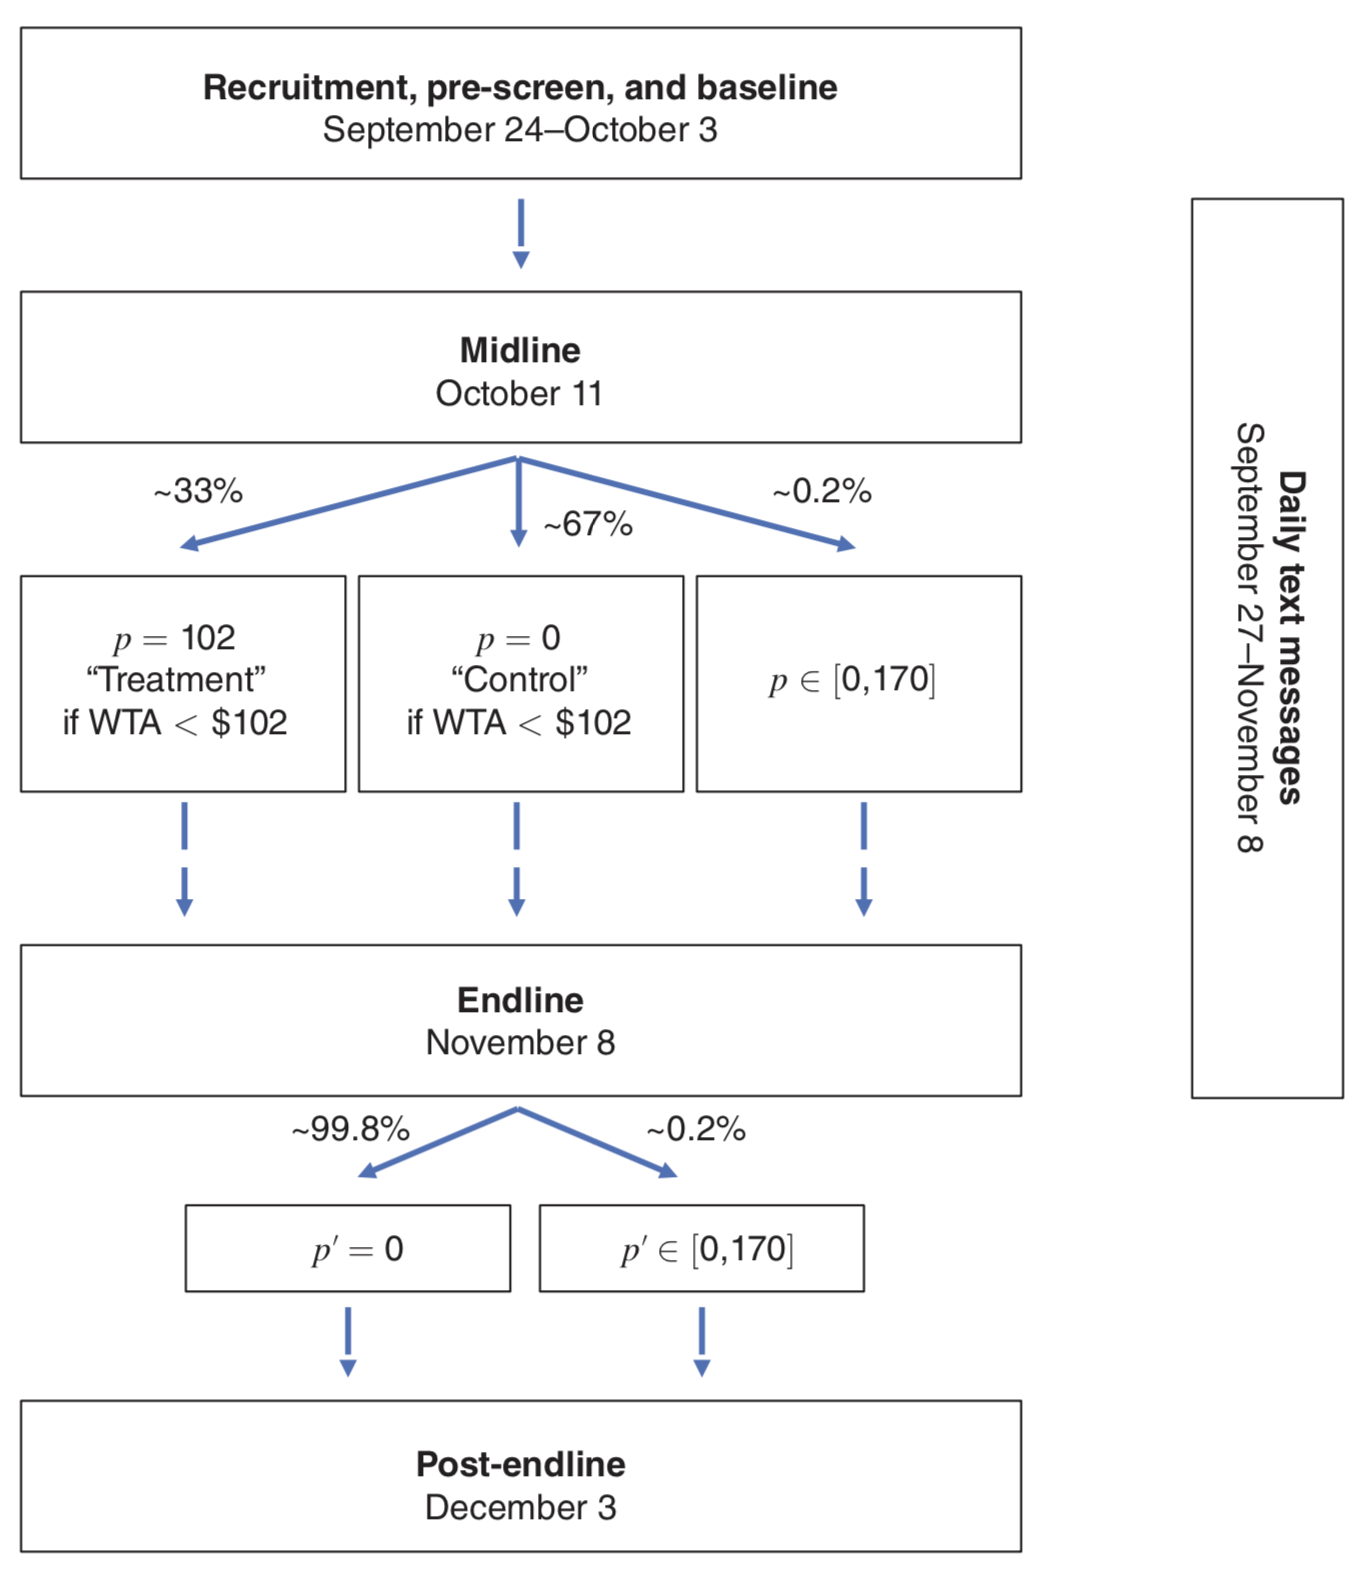
\includegraphics[width=\textwidth]{figures/allcott_welfare_2020_fig1}
\end{column}%

\hfill%

\begin{column}{.60\textwidth}
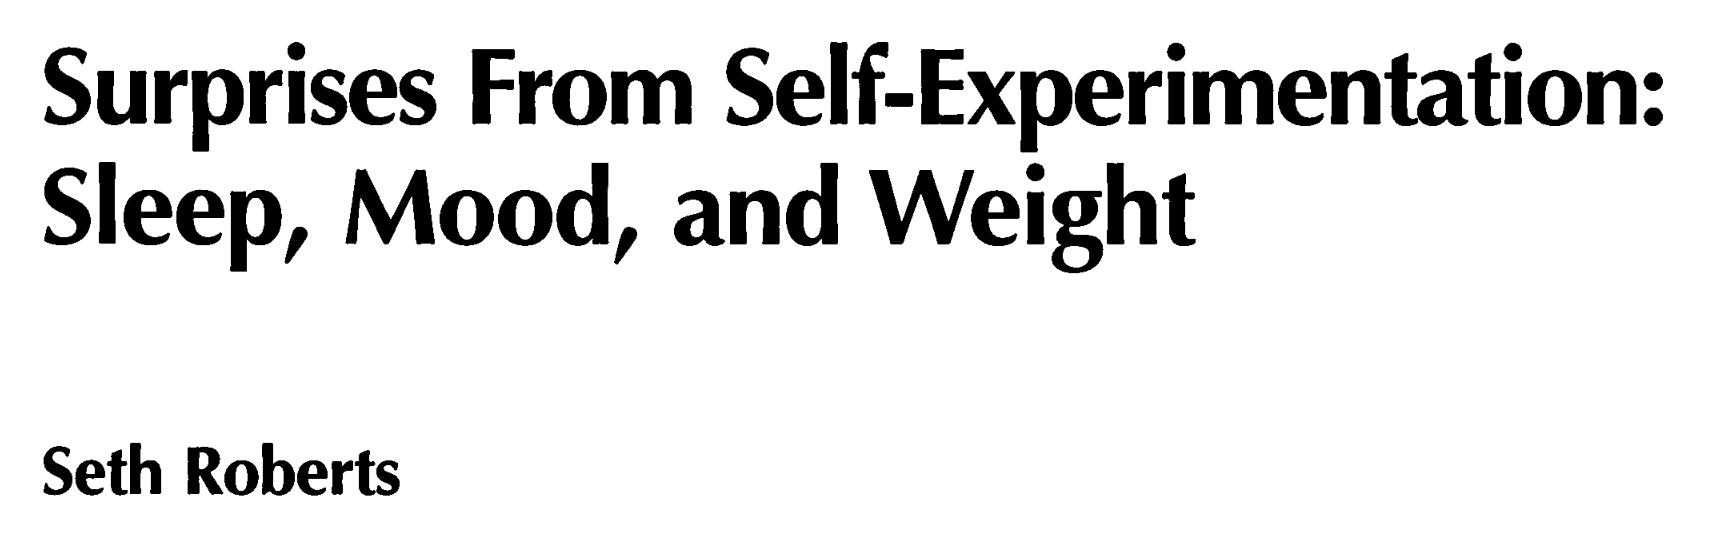
\includegraphics[width=\textwidth]{figures/roberts_surprises_2001_title}
\end{column}%
\end{columns}


\end{frame}
%%%%%%%%%%%%%%%%%%%
\begin{frame}

A few notes on self-experimentation
\begin{itemize}
\item Long history in medicine: {\tiny \url{https://en.wikipedia.org/wiki/Self-experimentation_in_medicine}} \pause
\item Not blinded \pause
\item Can't learn about heterogeneity across people \pause
\item Can learn about unexpected outcomes \pause
\item Can iterate quickly
\end{itemize}

\note{
Differences between self-experiment 
}
\end{frame}
%%%%%%%%%%%%%%%%%%%
\begin{frame}

\begin{columns}
\begin{column}{.40\textwidth}
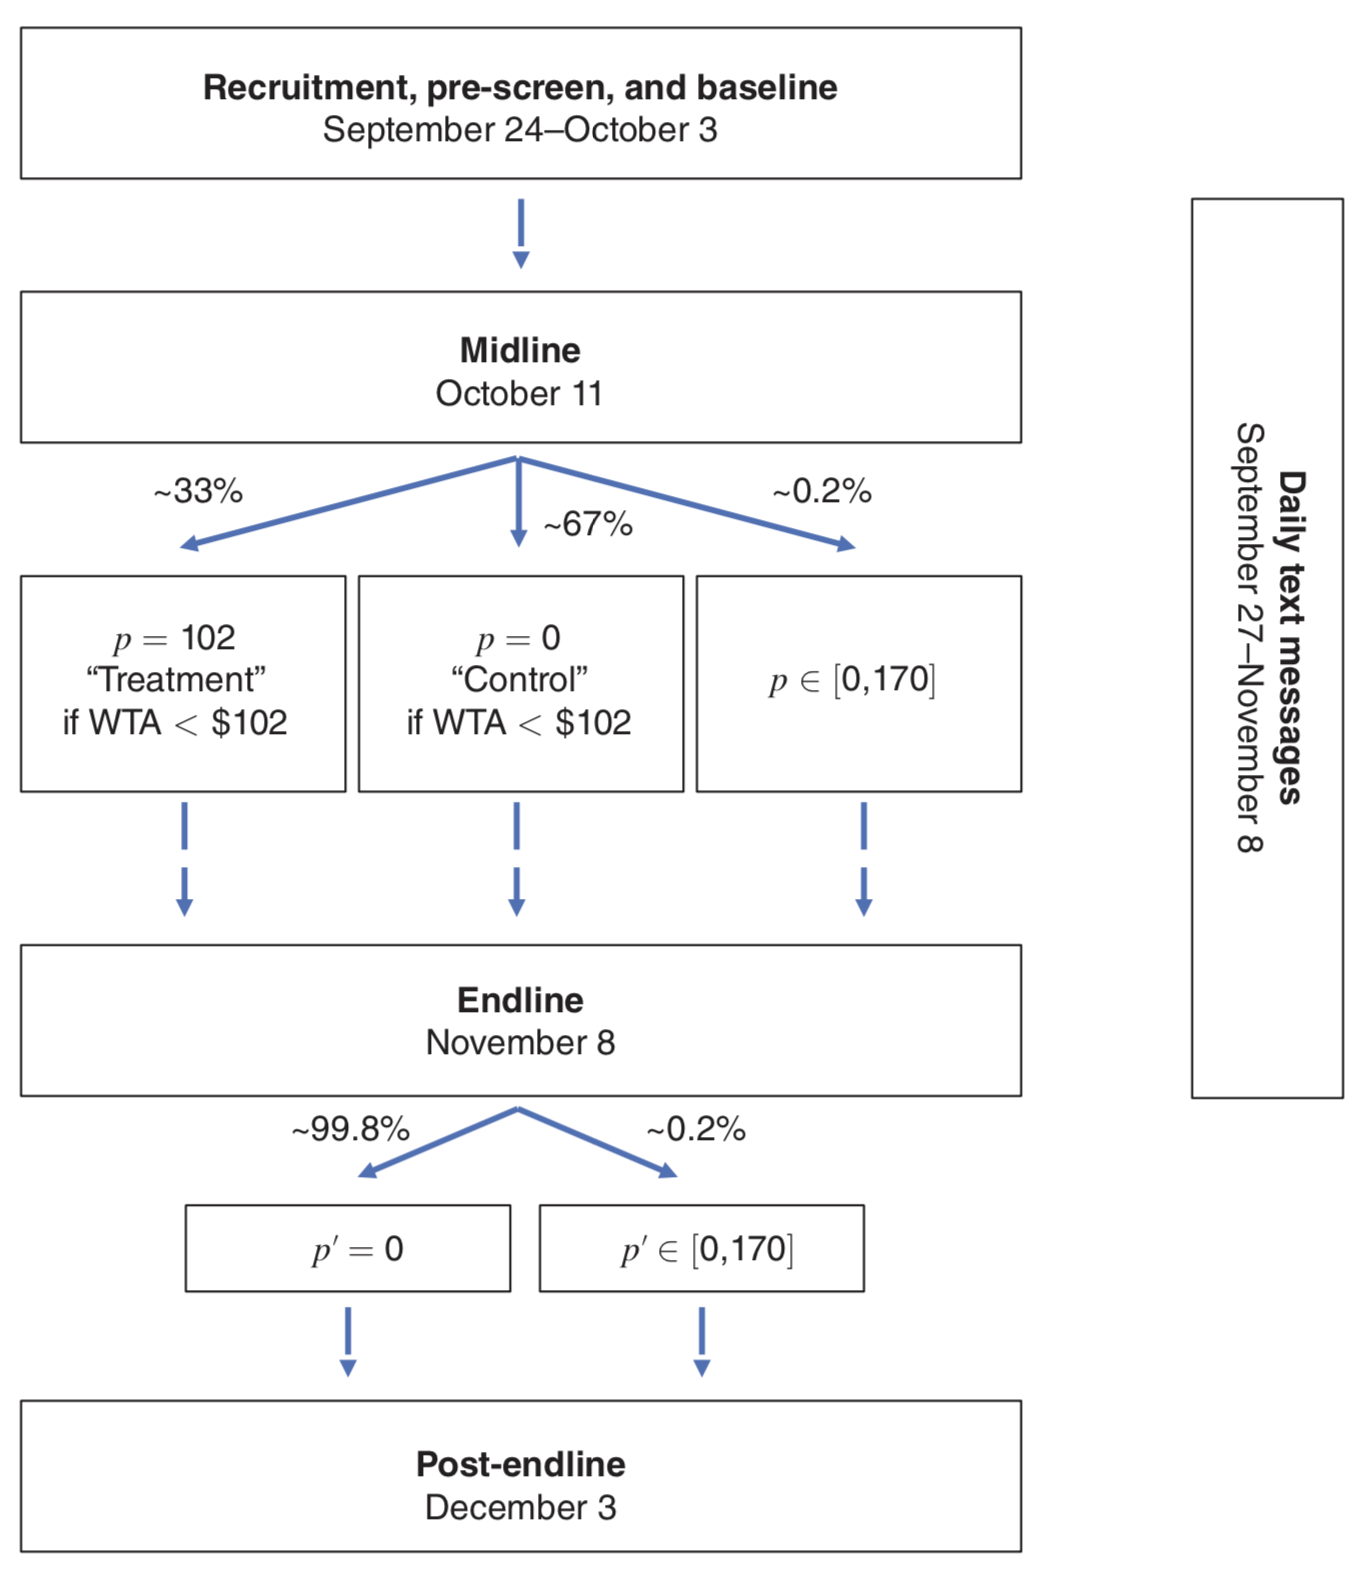
\includegraphics[width=\textwidth]{figures/allcott_welfare_2020_fig1}
\end{column}%

\hfill%

\begin{column}{.60\textwidth}
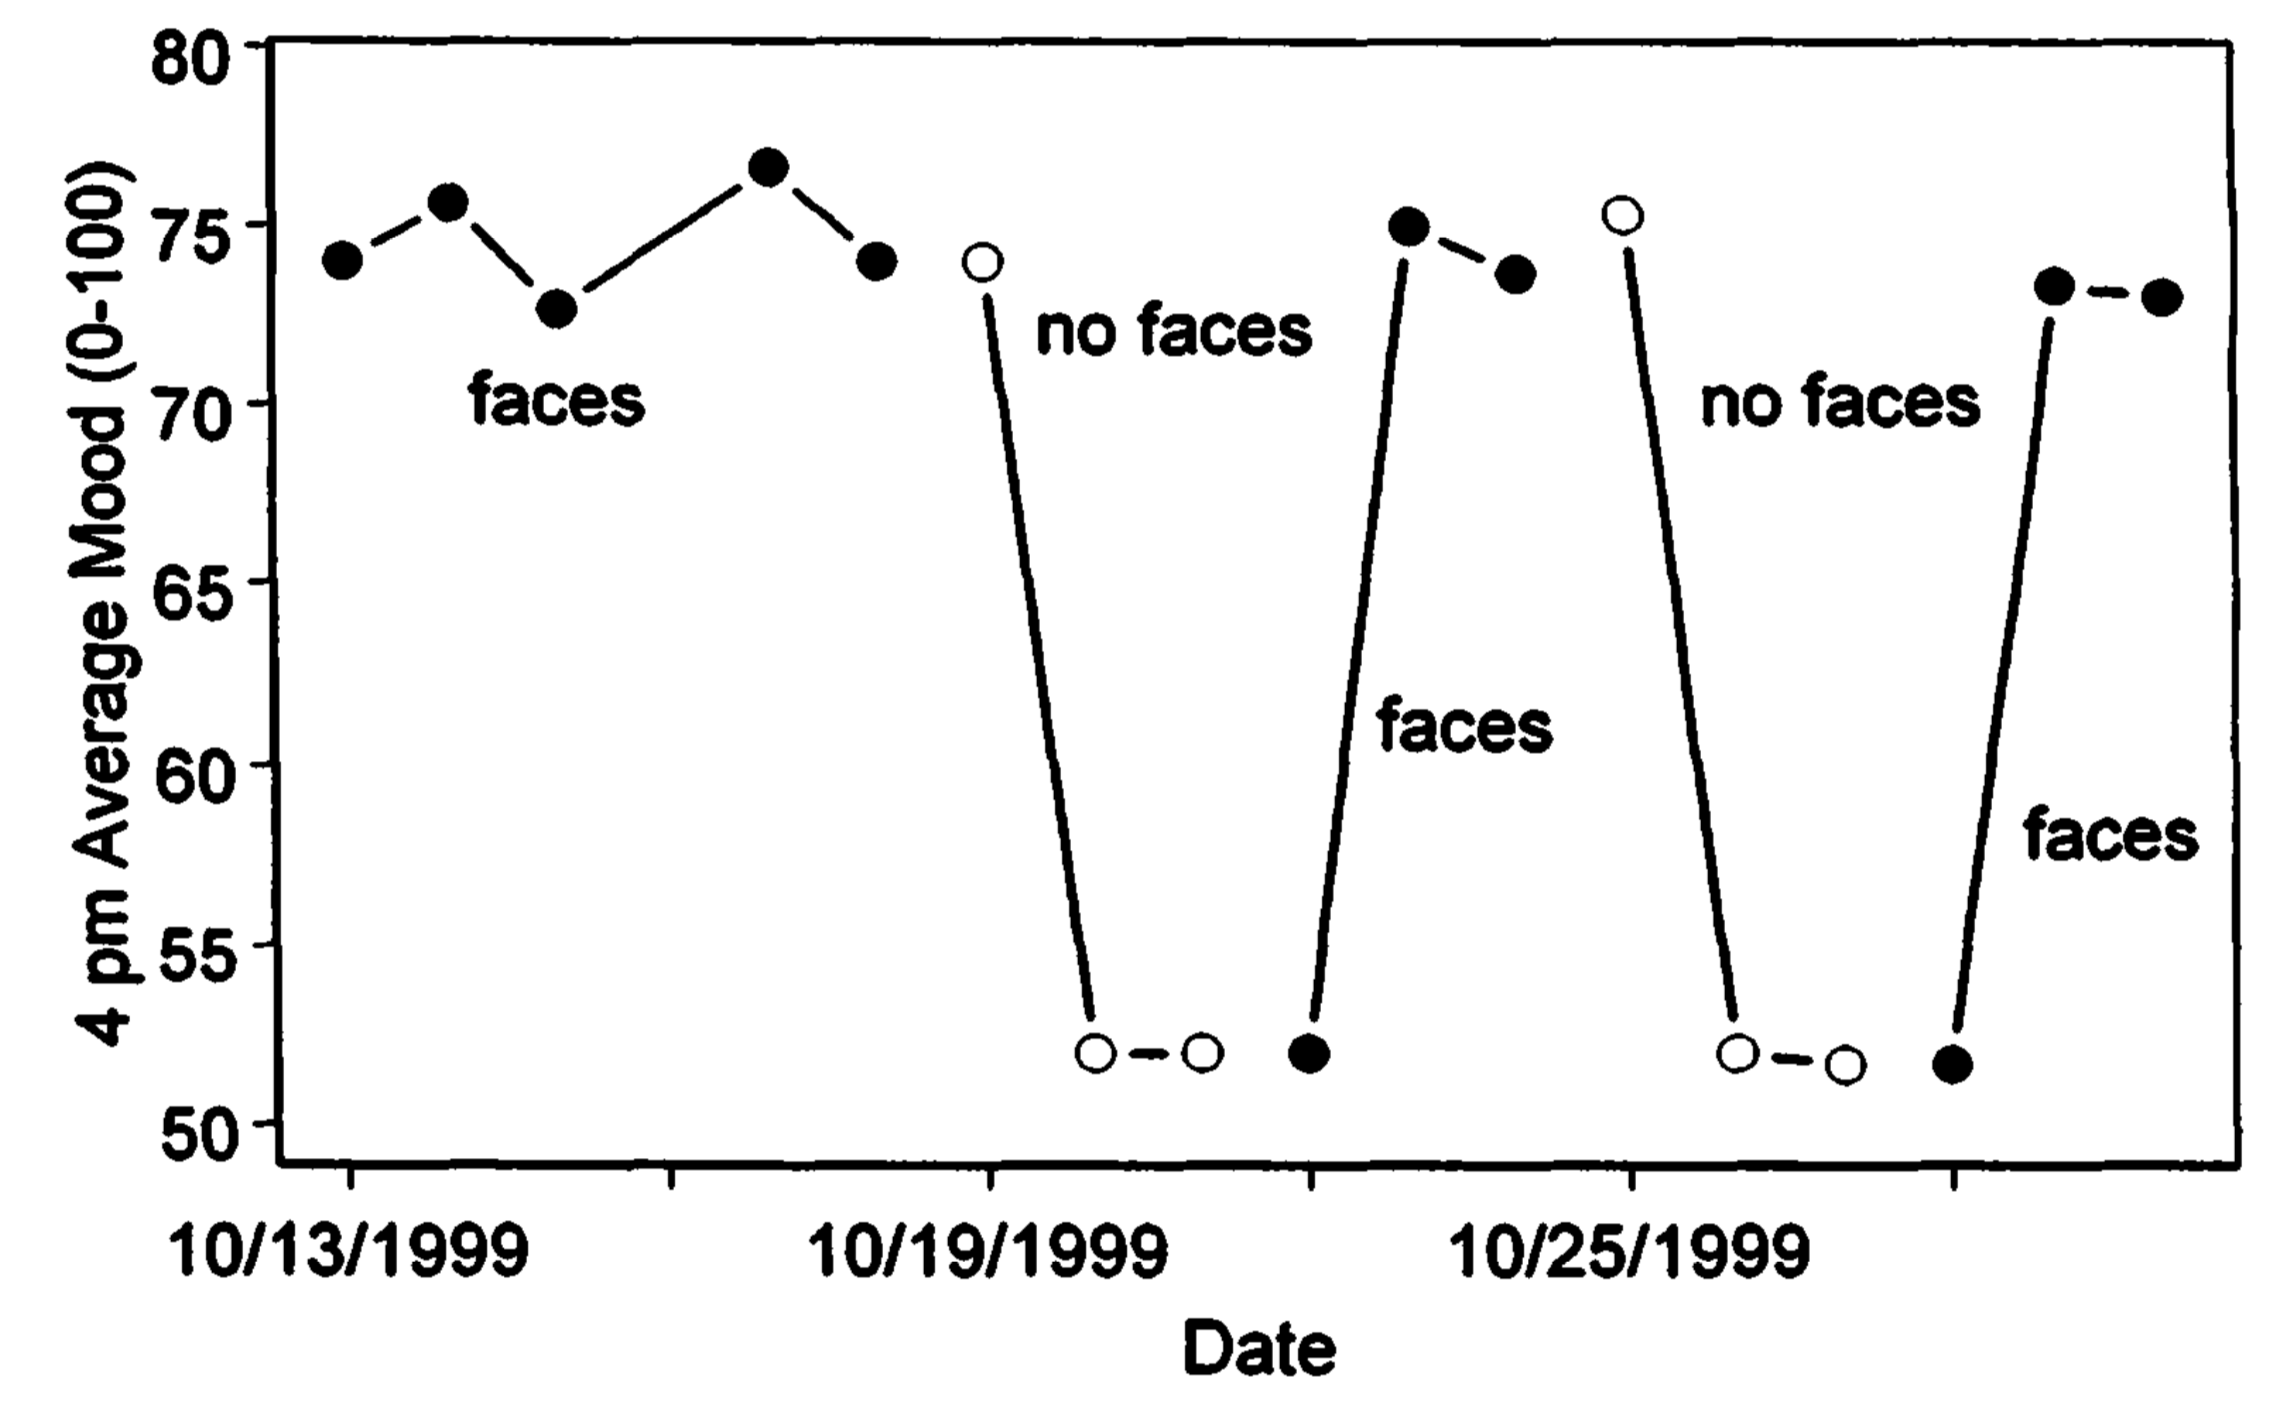
\includegraphics[width=\textwidth]{figures/roberts_surprising_2001_fig2upper}
\end{column}%
\end{columns}

\end{frame}
%%%%%%%%%%%%%%%%%%%
\begin{frame}

A few notes about this assignment:
\begin{itemize}
\item Choose an interesting and important intervention. Best ones will likely be either motivated by science or wellbeing. \pause
\item Have realistic expectations about what is feasible in a class assignment. \pause
\item You can stop your self-experimentation at any time, in fact you don't have to start. \pause
\item If this assignment causes problems, come talk to us or University Health Services.
\end{itemize}

\end{frame}
%%%%%%%%%%%%%%%%%%%
\begin{frame}

We look forward to seeing what you come up with

\end{frame}
%%%%%%%%%%%%%%%%%%%
\begin{frame}

Next class
\begin{itemize}
\item Crokett, M.J. (2017). Moral outrage in the digital age. \textit{Nature Human Behavior}.
\item Brady, W.J. et al. (2021). How social learning amplifies moral outrage expression in online social networks. \textit{Working paper}.
\item Aral, S. (2018). How lies spread online. \textit{New York Times}.
\item Vosoughi, S. et al. (2018). The spread of true and false news online. \textit{Science}.
\item Lazer, D. (2015). The rise of the social algorithm. \textit{Science}.
\item Bakshy, E., Messing, S., and Adamic, L.A. (2015) Exposure to ideologically diverse news and opinion on Facebook. \textit{Science}. 
\end{itemize}

\end{frame}
%%%%%%%%%%%%%%%%%%%



\end{document}
